\documentclass{article}

\usepackage[utf8]{inputenc}
\usepackage[top=1.5in,left=.9in,right=.9in,bottom=1in,headheight=1in]{geometry}
\usepackage{fancyhdr}
\usepackage{lastpage}
\usepackage{amsmath,amssymb,amsthm}
\usepackage{mathrsfs}
\usepackage{multicol}
\usepackage{enumerate}

\usepackage{tkz-graph}
\usetikzlibrary{arrows}



% Better looking empty set
\let\emptyset\varnothing

\newtheoremstyle{problem}{\topsep}{\topsep}%
{}%         Body font
{}%         Indent amount (empty = no indent, \parindent = para indent)
{\bfseries}% Thm head font
{\vspace{5pt}}%        Punctuation after thm head
{\newline}%     Space after thm head (\newline = linebreak)
{\thmname{#1}\thmnote{ #3}}%         Thm head spec

\theoremstyle{problem}
\newtheorem{prob}{Problem}

\theoremstyle{plain}
%\newtheorem{thm}{Theorem}
\newtheorem{lem}{Lemma}
\newtheorem{prop}{Proposition}
% No indent for whole page
\setlength\parindent{0pt}

\theoremstyle{remark}
\newtheorem{countex}{Counterexample}

\setlength{\columnsep}{1cm}
%%% Heading -- No need to edit %%%
\pagestyle{fancy}

\rhead{
  Stefan Eng\\
  Dr. Katherine Stevenson\\
  Math 320\\
  10/16/13
}
\lhead{
  Ch 4: \# 10, 11, 13, 19, 20, 25, 34
}

\cfoot{Page\ \thepage\ of\ \pageref{LastPage}}

%%%

\renewcommand{\qedsymbol}{$\blacksquare$}
% For manual qed box
\def\bs{\hspace{\stretch1}\ensuremath\blacksquare}

\begin{document}

%%% Make the title %%%
\begin{center}
\textsc{\Large Foundations of Higher Mathematics}\\[.3cm]
\textsc{\Large Homework 7}
\end{center}
%%% End title %%%

%%% Start Assignment Here %%%
\begin{prob}[10]\ \\[-1cm]
  \begin{proof}
    $(\subseteq)$ Let $x \in A \cup B$ and $x \not \in A \cap B \cap C$. Then $x \not \in A$ or $x \not \in B$ or $x \not \in C$ by De Morgan's law. Suppose $x \in A$. Then $x \not \in B$ or $x \not \in C$. It follows that $x \not \in B \cap C$, and thus, $x \in A - (B \cap C)$. So, $x \in [A - (B \cap C)] \cup [B - (A \cap C)]$. Now suppose the $x \in B$. Then $x \not \in A$ or $x \not \in C$. Thus, $x \not \in A \cap C$. It follows that $x \in B - (A \cap C)$, and thus $x \in [A - (B \cap C)] \cup [B - (A \cap C)]$.\\

    $(\supseteq)$ Let $x \in [A - (B \cap C)] \cup [B - (A \cap C)]$. Suppose $x \in A - (B \cap C)$. Then $x \in A$ and $x \not \in B$ or $x \not \in C$. It follows that $x \in A$ or $x \not \in A$. Similarly, $x \not \in B$ or $x \in B$. By De Morgan's Law, $x \not \in A \cap B \cap C$. Since $x \in A$ not $x \in B$ and $x \not \in A \cap B \cap C$, $(A \cup B) - (A \cap B \cap C)$. Now suppose that $x \in B - (A \cap C)$. Then $x \in B$ and $x \not \in (A \cap C)$. It follows that $x \not \in A$ or $x \not \in C$. Since $x \in B$ then $x \in B \cup A$. Also, $x \in B$ or $x \not \in B$. Then $x \not \in A$ or $x \not \in B$ or $x \not \in C$ and thus $x \not \in A \cap B \cap C$. Therefore, $x \in (A \cup B) - (A \cap B \cap C)$.
  \end{proof}
\end{prob}
%

\begin{prob}[11]\ \\[-1cm]
\begin{enumerate}[a)]
\item \begin{proof}
Suppose $S \subseteq T$ and $x$ is in the domain of $S$. Then for an arbitrary element $y \in S[x]$, $(x,y) \in S$. Since $S \subseteq T$ and $(x,y) \in S$, then $(x,y) \in T$ and $y \in T[x]$. Therefore, $S[x] \subseteq T[x]$.
\end{proof}
\item \begin{itemize}
    \item $(A \times B)[x] = B$ if $x \in A$. 
\begin{proof}
($\subseteq$) If $x \in A$ and $y \in (A \times B)[x]$, then $(x,y) \in (A \times B)$. It follows that $y \in B$ from the definition of the Cartesian Product. Therefore, $(A \times B)[x] \subseteq B$.\\
($\supseteq$) If $x \in A$ and $y \in B$ then $(x,y) \in (A \times B)$. It follows that $y \in (A \times B)[x]$. Therefore, $B \subseteq (A \times B)[x]$.
\end{proof}
\item $(A \times B)[x] = \emptyset$
\begin{proof}
($\supseteq$) $\emptyset$ is the subset of every set, therefore $\emptyset \subseteq (A \times B)[x]$.\\
($\subseteq$) If $x \not \in A$ and $y \in (A \times B)[x]$ Since $x$, and arbitrary element, is not in the domain $A$ then $(A \times B)[x]$ is not defined and thus, it is vacuously true that $y \in \emptyset$ so $(A \times B)[x] \subseteq \emptyset$.
\end{proof}
\end{itemize}
\end{enumerate}
\end{prob}
%

\begin{prob}[13]
$R[7] = \{7,14,21,28,35,\ldots \}$
\\[5pt]
$R[14] = \{14,28,42,56,70,\ldots \}$
\\[5pt]
The only $n \in \mathbb{N}$ for which $R[n] = \mathbb{N}$ is $n = 1$.

\end{prob}
%

\begin{prob}[19]
Given the relation $A = \{(1,1), (1,2), (1,3), (3,4), (4,1), (4,3), (4,5), (5,2),(5,4)\}$ the Cartesian graph looks like:\\
\begin{center}
  \begin{tikzpicture}

    \foreach \x in {1,...,5} \foreach \y in {1,...,5} \fill (\x,\y) circle (1pt);

    %(1,1)
    \draw (1,1) circle (3pt);
    %(1,2)
    \draw (1,2) circle (3pt);
    %(1,3)
    \draw (1,3) circle (3pt);
    %(3,4)
    \draw (3,4) circle (3pt);
    %(4,1)
    \draw (4,1) circle (3pt);
    %(4,3)
    \draw (4,3) circle (3pt);
    %(4,5)
    \draw (4,5) circle (3pt);
    %(5,2)
    \draw (5,2) circle (3pt);
    %(5,4)
    \draw (5,4) circle (3pt);

  \end{tikzpicture}
\end{center}
\end{prob}
%

\newpage

\begin{multicols}{2}
\begin{prob}[20a]
  $R = \{(a,b) \in A \times A:a\text{ divides } b\}$\\[5pt]

  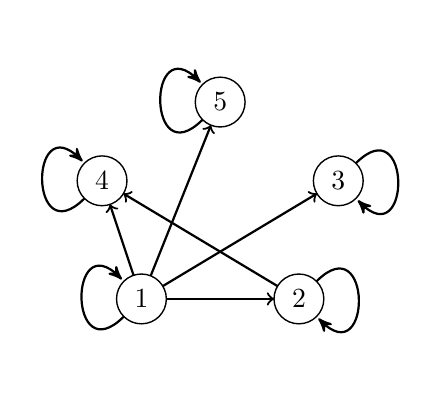
\begin{tikzpicture}
    % Vertices
    \Vertex[x=-1, y=0]{1}
    \Vertex[x=1, y=0]{2}
    \Vertex[x=1.5, y=1.5]{3}
    \Vertex[x=-1.5, y=1.5]{4}
    \Vertex[x=0, y=2.5]{5}

    % Edges
    \tikzset{EdgeStyle/.append style = {-> }}
    % 1 | everything
    \Edge(1)(2) 
    \Edge(1)(3) 
    \Edge(1)(4) 
    \Edge(1)(5) 
    

    % 2 | 4 
    \Edge(2)(4)

    % 3 | 


    % Loops
    \Loop[dist=1cm](1)
    \Loop[dist=1cm,dir=EA](2)
    \Loop[dist=1cm,dir=EA](3)
    \Loop[dist=1cm](4)
    \Loop[dist=1cm](5)

  \end{tikzpicture}
\end{prob}

\begin{prob}[20b]
  $U = \{(a,b) \in A \times A:a \not = b\}$\\[5pt]
  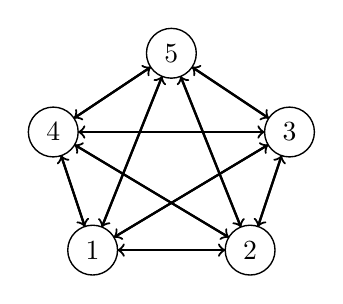
\begin{tikzpicture}
    % Vertices
    \Vertex[x=-1, y=0]{1}
    \Vertex[x=1, y=0]{2}
    \Vertex[x=1.5, y=1.5]{3}
    \Vertex[x=-1.5, y=1.5]{4}
    \Vertex[x=0, y=2.5]{5}

    % Edges
    \tikzset{EdgeStyle/.append style = {-> }}
    
    % (1,b)
    \foreach \x in {2,...,5} \Edge(1)(\x);

    % (2,b)
    \foreach \x in {3,...,5} \Edge(2)(\x);
    \Edge(2)(1);

    % (3,b)    
    \foreach \x in {4,...,5} \Edge(3)(\x);
    \foreach \x in {1,...,2} \Edge(3)(\x);

    % (4,b)
    \foreach \x in {1,...,3} \Edge(4)(\x);
    \Edge(4)(5);

    % (5,b)
    \foreach \x in {1,...,4} \Edge(5)(\x);

  \end{tikzpicture}
\end{prob}
\vfill
\columnbreak

\begin{prob}[20c]
  $E = \{(a,b) \in A \times A:a + b \text{ is even}\}$\\[5pt]
  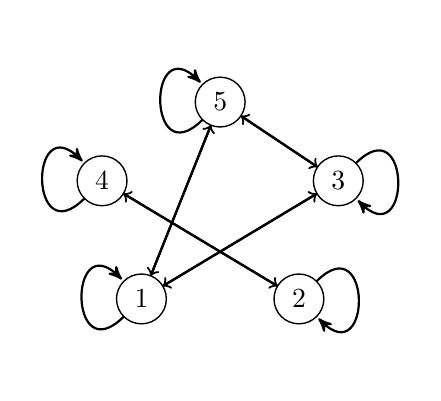
\begin{tikzpicture}
    % Vertices
    \Vertex[x=-1, y=0]{1}
    \Vertex[x=1, y=0]{2}
    \Vertex[x=1.5, y=1.5]{3}
    \Vertex[x=-1.5, y=1.5]{4}
    \Vertex[x=0, y=2.5]{5}

    % Edges
    \tikzset{EdgeStyle/.append style = {-> }}
    
    \foreach \x in {1,3,...,5} \foreach \y in {1,3,...,5} \ifthenelse{\equal{\x}{\y}}{}{\Edge(\x)(\y)};

    \foreach \x in {2,4} \foreach \y in {2,4} \ifthenelse{\equal{\x}{\y}}{}{\Edge(\x)(\y)};
%    \Edge(1)(2) 

    % Loops
    \Loop[dist=1cm](1);
    \Loop[dist=1cm](4);
    \Loop[dist=1cm](5);
    
    \Loop[dist=1cm,dir=EA](2);
    \Loop[dist=1cm,dir=EA](3);

  \end{tikzpicture}
\end{prob}

\begin{prob}[20d]
  $O = \{(a,b) \in A \times A:a + b \text{ is odd}\}$\\[5pt]
  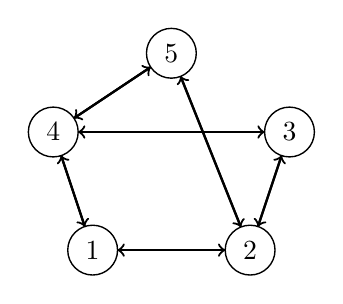
\begin{tikzpicture}
    % Vertices
    \Vertex[x=-1, y=0]{1}
    \Vertex[x=1, y=0]{2}
    \Vertex[x=1.5, y=1.5]{3}
    \Vertex[x=-1.5, y=1.5]{4}
    \Vertex[x=0, y=2.5]{5}

    % Edges
    \tikzset{EdgeStyle/.append style = {-> }}
    \foreach \x in {1,3,...,5} \foreach \y in {2,4} \ifthenelse{\equal{\x}{\y}}{}{\Edge(\x)(\y)};

    \foreach \x in {2,4} \foreach \y in {1,3,...,5} \ifthenelse{\equal{\x}{\y}}{}{\Edge(\x)(\y)};
  \end{tikzpicture}
\end{prob}
% 
\end{multicols}


\begin{prob}[25]

\end{prob}
%

\begin{prob}[34]\ \\[-1cm]
\begin{multicols}{2}
\begin{enumerate}[a)]
\item \textbf{Non Reflexive:} $1 \in \mathbb{R}$ but $1 \cdot 1 \not = 0$ and thus $(1,1) \not \in R_1$\\
  \textbf{Symmetric:} Suppose $(x,y) \in R_1$. Then $xy = 0$ and $yx = 0$. Thus $(y,x) \in R_1$. Therefore, $R_1$ is Symmetric.\\
  \textbf{Non Transitive:} $1 \cdot 0 = 0$ so $(1,0) \in R_1$. $0 \cdot 1 = 0$ so $(0,1) \in R_1$ but $1 \cdot 1 \not = 0$ so $(1,1) \not \in R_1$.
\item \textbf{Reflexive:} Suppose $x \in \mathbb{R}$. Then, $|x - x| = 0 < 5$ so $(x,x) \in R_2$.\\
  \textbf{Symmetric:} Suppose $(x,y) \in R_2$. Then $|x - y| < 5$. It follows that, $|-(y - x)| < 5$ and $|y - x| < 5$. Therefore, $(y,x) \in R_2$ so $R_2$ is symmetric.\\
  \textbf{Non Transitive:} $|10 - 6| < 5$ and $|6 - 2| < 5$ so $(10,6) \in R_2$ and $(6,2) \in R_2$ but $|10 - 2| = 8 \not < 5$.
\item \textbf{Non Reflexive:} $0 \in \mathbb{R}$ but $0 \cdot 0 = 0$.\\
\textbf{Symmetric:} Suppose $(x,y) \in R_3$. Thus, $xy \not = 0$. It follows that $yx \not = 0$ so $(y,x) \in R_3$. Therefore, $R_3$ is symmetric.\\
\textbf{Transitive:} (Contrapositive) Suppose $(x,z) \not \in R_3$. Then $xz = 0$. So either $x = 0$ or $z = 0$. Assume $x = 0$. Then $xy = 0$, and $(x,y) \not \in R_3$. So $(x,y) \not \in R_3$ or $(y,z) \not \in R_3$ by disjunction introduction. Now assume, $z = 0$. It follows that $yz = 0$. So, $(y,z) \not \in R_3$ or $(x,y) \not \in R_3$. Therefore, by the contrapositive, $R_3$ is transitive.
Suppose $(x,y) \in R_3$ and $(y,z) \in R_3$.
\item \textbf{Reflexive:} Let $x \in \mathbb{R}$. Then $x \geq x$ so $(x,x) \in R_4$.\\
  \textbf{Non Transitive:} $2 \geq 1$ so $(2,1) \in R_4$ but $1 < 2$ so $(1,2) \not \in R_4$.\\
  \textbf{Transitive:} Suppose $(x,y) \in R_4$ and $(y,z) \in R_4$. So $x \geq y$ and $y \geq z$. It follows that, $x \geq y \geq z$ and thus, $x \geq z$. Hence, $(x,z) \in R_4$.
\item \textbf{Non Reflexive:} $1 \in \mathbb{R}$ but $1^2 + 1^2 = 2 \not = 1$.\\
  \textbf{Symmetric:} Suppose $(x,y) \in R_5$. So $x^2 + y^2 = 1$. It follows that $y^2 + x^2 = 1$ so $(y,x) \in R_5$\\
  \textbf{Non Transitive:} $1^2 + 0^2 = 1$ so $(1,0) \in R_5$ and $0^2 + 1^2 = 1$ so $(0,1) \in R_5$ but $1^1 + 1^1 = 2 \not = 1$ so $(1,1) \not \in R_5$.
\end{enumerate}
\end{multicols}
\end{prob}

% 

\end{document}